% !TEX program = lualatex
\documentclass[11pt]{article}
\usepackage[utf8]{inputenc}
\usepackage{graphicx}
\usepackage{amsmath}
\usepackage{hyperref}
\usepackage{caption}
\usepackage{subcaption}
\usepackage{geometry}
\usepackage{float}
\usepackage{pdfpages}
\usepackage{pifont}
\usepackage{todonotes}
\usepackage{booktabs}
\usepackage{array}
\usepackage{enumitem}
\usepackage{setspace}


\geometry{margin=2.5cm}
\sloppy
\onehalfspacing


\title{CreaRobot}
\author{Marco Grandclaude}
\date{\today}

\begin{document}

\begin{titlepage}
    \centering
    
    \centering
    % Logos
    \begin{minipage}{0.45\textwidth}
        
\includegraphics[height=2cm]{figures/logo_sorbonne.png}\\[0.3cm]
        
\includegraphics[height=2cm]{figures/logo_polytech.png}
    \end{minipage}
    \hfill
    \begin{minipage}{0.45\textwidth}
        \raggedleft
        
\includegraphics[height=1cm]{figures/logo_lutin.png}
    \end{minipage}
    
    \vspace{3cm}
    
    % Title
    {\Huge \textbf{CreaRobot}} \\[1cm]
    {\Large Rapport de Stage Technique} \\[2cm]
    
    % Info autor
    {\Large Marco Grandclaude} \\[0.5cm]
    {\large Sorbonne Université – Polytech Sorbonne} \\[0.3cm]
    {\large Robotique } \\[0.3cm]
    {\large 2025–2026} \\[2cm]
    
    % Info Stage
    {\large 1er mars, 2025 – 31 août, 2026} \\[0.5cm]
    {\large Laboratoire CHART} \\[2cm]
    
    % Bottom
    \vfill
    {\large Paris, \today}
\end{titlepage}
\newpage

\pagenumbering{gobble}

% Abstract
\begin{center}
    \Huge \textbf{Abstract}
\end{center}
\vspace{0.5cm}
\newpage

% Acknowledgments
\begin{center}
    \Huge \textbf{Remerciements}
\end{center}
\vspace{0.5cm}
Je tiens à remercier sincèrement ma famille, mes parents, mes frères et ma sœur pour leur soutien tout au long de mes études et de ce stage.

Je remercie également mon tuteur académique, Mahdi Khoramshahi, pour son implication dans le suivi de ce projet et pour avoir assuré le cadre pédagogique de ce travail de recherche.

Ma profonde gratitude s'adresse à mon maître de stage, Salvatore Anzalone, pour son mentorat, ses précieux conseils et l'accompagnement constant qu'il m'a apporté tout au long de cette expérience.

Je tiens à adresser un merci tout particulier à Claudie Cuveillier pour notre collaboration au sein de ce partenariat. Son travail sur la dimension sciences cognitives a été fondamental pour la réussite du projet et je la remercie pour cette synergie extrêmement productive.

Je souhaite aussi remercier Geoffrey Tissier, responsable technique de la plateforme, pour son aide précieuse, ainsi que les doctorants et les autres stagiaires pour nos échanges enrichissants et la collaboration qui a rendu ce stage très agréable.

Enfin, je remercie le laboratoire pour son accueil et pour m'avoir permis d'évoluer au sein d'un environnement scientifique aussi stimulant et propice à l'innovation.
\newpage

\tableofcontents
\newpage
\pagenumbering{arabic}

\listoffigures
\newpage
\listoftables
\newpage

% ============================================================
\section{Introduction}

\subsection{Contexte du stage}

Ce rapport présente le travail réalisé dans le cadre d'un stage technique effectué au sein du
laboratoire CHART, sur la plateforme Lutin, du 1\textsuperscript{er} mars 2025 au 31 août 2026.
Ce stage s'inscrit dans le cursus ingénieur de la filière Robotique de Polytech Sorbonne
(Sorbonne Université), en troisième année de cycle ingénieur.

Le stage a été encadré par Salvatore Anzalone, maître de stage et chercheur à CHART, ainsi que
par Mahdi Khoramshahi, tuteur académique à Polytech Sorbonne.
Le travail a été mené en collaboration étroite avec Claudie Cuveillier, stagiaire en ergonomie, qui a notamment pris en charge la conception des protocoles de dialogue pour le robot.

\subsection{Présentation du laboratoire CHART et de la plateforme Lutin}

Le laboratoire CHART (Cognitions Humaines et Artificielles) est une unité mixte de recherche.
Ses travaux portent sur les interactions entre cognition humaine et systèmes numériques, à
l'interface de la psychologie cognitive, des sciences de l'éducation et de l'intelligence
artificielle.

La plateforme Lutin est rattachée au laboratoire CHART et constitue son infrastructure expérimentale.
Le LUTIN (Laboratoire des Usages en Technologies d'Information Numériques) contrairement à
ce que son nom indique n’est pas un laboratoire mais est une plateforme de recherche collaborative 
et pluridisciplinaire dédiée à l'étude des sciences cognitives et de la robotique, dont l'ambition 
est d'explorer la relation entre l'humain et le numérique dans le cadre académique mais aussi industriel. 
C'est un endroit où l'on étudie comment les gens utilisent les technologies, pour mieux les concevoir, les évaluer et, 
in fine, les mettre au service des utilisateurs. 
Le LUTIN est dirigé par Salvatore Anzalone, avec Ugo Ballenghein en tant que directeur adjoint,
tous deux membres du laboratoire CHArt.
Le LUTIN vise à développer des connaissances et des méthodes dans le champ des usages et des pratiques numériques, quels qu’en soient les domaines d’application. Pour ce faire, il dispose d’un parc d’équipements technologiques permettant l’analyse de mesures comportementales et neurophysiologiques en temps réel : eye-tracking, EEG, motion capture, réalité virtuelle, robotique ou encore dispositif de vitres sans tain pour observer les potentiels participants dans des cadres écologiques. Ces outils permettent d’aller bien au-delà du simple questionnaire et d’investiguer au mieux les comportements réels des utilisateurs face à une technologie.

\subsection{Le projet CreaRobot : objectifs et enjeux}

Le projet CreaRobot pose une question de recherche centrale : un robot social peut-il, par
l'interaction, améliorer la créativité d'une personne en train de dessiner ?

Pour répondre à cette question, l'expérience repose sur le test de créativité TCT-DP
(\textit{Test for Creative Thinking – Drawing Production}, Urban, 1991), un test standardisé
consistant à compléter une figure géométrique partielle. Le protocole compare trois conditions
expérimentales : un feedback neutre délivré par le robot (condition de contrôle), un échange piloté par un modèle de langage mêlant questions, suggestions et idées portant sur le dessin du participant (condition C1), et un retour visuel génératif projeté
sur la zone de dessin (condition C2).

L'enjeu technique de ce stage est de concevoir et développer de A à Z le système logiciel
permettant au robot social QTRobot (plateforme ROS\,1 / Python\,2.7) d'interagir en temps réel
avec des participants humains, en s'appuyant sur une intelligence déportée sur un PC externe
(ROS\,2 / Python\,3) : reconnaissance vocale, traitement du langage naturel, pilotage des
expressions et des gestes, synchronisation avec les phases du protocole.

Le système a fait l'objet d'une première passation lors de la Semaine de la Science Infuse,
qui constitue une phase pilote exploratoire. Une passation principale est prévue en juin 2026.
Le robot utilisé dans ce projet est illustré en figure~\ref{fig:qtrobot}.

\begin{figure}[H]
    \centering
    \vspace{0.3cm}
    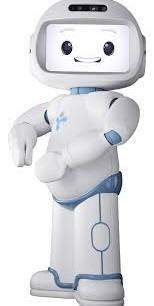
\includegraphics[height=10cm]{figures/qtrobot.jpeg}
    \caption{Le robot social QTRobot.}
    \label{fig:qtrobot}
\end{figure}

\newpage

% ============================================================
\section{Contexte scientifique}
% Note : garder cette partie concise, pas le cœur du rapport technique.

\subsection{Robotique sociale et interaction homme-robot}
\subsection{La créativité et le test TCT-DP}
% Présentation rapide du TCT-DP (Urban, 1991) — les détails du protocole
% sont en section~\ref{sec:protocole}.
\subsection{État de l'art : robots sociaux dans des protocoles expérimentaux}
% Quelques références sur l'usage de robots sociaux en recherche cognitive.
% Rester bref, on ne sait pas encore exactement ce que ça va contenir.

\newpage

% ============================================================
\section{Présentation du robot QTRobot}

\subsection{Architecture matérielle et logicielle}
% QTRobot V1 (Hyppolite) — Linux, ROS 1 Kinetic, Python 2.7
% Deux PC internes (face/torse), ReSpeaker, caméra RealSense, caméra USB
\subsection{Prise en main : fonctionnalités de base}
% Parole (qt_robot/speech/say), émotions, gestes, audio, behaviors
% Connexion SSH, scp, rqt_image_view, web interface port 8080
% Nuitrack hand tracking — résolution du conflit caméra USB / capteur 3D
\subsection{Contraintes et limites de la plateforme}
% OS vieux → pas de remote SSH VSCode → solution SSHFS
% Dépendances Python 2/3 : enfer des bibliothèques (ex. vosk, requests)
% Versions du software LuxAI non disponibles → certains modules absents
% ou non fonctionnels selon la version du robot (travail sur 2 versions)
% Ex. qt_vosk_app : présent dans les fichiers mais inutilisable

\newpage

% ============================================================
\section{Le protocole expérimental TCT-DP}
\label{sec:protocole}
% Placé avant l'architecture pour donner au lecteur le contexte
% qui justifie chaque choix technique.

\subsection{Description du test de créativité TCT-DP}
\subsection{Les cinq phases de l'expérience}
% Schéma visuel simple (timeline) — pas de détail technique ici,
% c'est développé dans la partie développement.
\subsection{Les trois conditions expérimentales}
\subsubsection{Condition C0 : feedback neutre (groupe contrôle)}
\subsubsection{Condition C1 : dialogue socratique piloté par le LLM}
% Prompt de Claudie — interaction ouverte pendant les phases de dessin
\subsubsection{Condition C2 : feedback visuel génératif (projection)}
% Implémentée mais non testée lors de la première passation.
% Incertitude sur son inclusion dans la passation de juin.
\subsection{Population cible et critères de scoring TCT-DP}
% Enfants, jeunes enfants, adolescents, adultes
% Critères : Ne, Cl, Cn, Pe, Cm, Cth, Uc\_b/d/c, Bfi/d, Hu Tableau existants

\newpage

% ============================================================
\section{Architecture technique du système CreaRobot}

% Intro de section : avant d'aboutir à l'architecture finale, une première
% approche a consisté à garder toute l'intelligence sur le robot lui-même —
% utiliser son micro ReSpeaker et sa caméra intégrée. Cette piste a été
% abandonnée pour plusieurs raisons :
% (1) Qualité du micro : en présence de bruit ambiant, la reconnaissance
%     vocale était instable. Les outils de filtrage proposés par LuxAI
%     (ex. qt_vosk_app) ne sont pas fonctionnels sur toutes les versions
%     du robot, et les anciennes versions du software ne sont plus
%     téléchargeables — rendant toute mise à jour impossible.
% (2) Dépendances Python 2 / Python 3 : tenter d'installer des libs récentes
%     sur le robot crée des conflits insolubles.
% (3) Caméra : fixée sur la tête de QT, elle ne peut pas photographier un
%     dessin posé sur une table sans que le participant ne le soulève.
% Solution retenue : externaliser les capteurs sur le PC (micro cravate USB
% + caméra externe) et y concentrer toute l'intelligence du système.

\subsection{Tentative initiale : capteurs embarqués sur le robot}
% Développer les raisons ci-dessus en prose

\subsection{Solution retenue : externalisation sur le PC ROS\,2}
% Avantages : qualité audio, indépendance du robot, portabilité vers
% d'autres QTRobots sans reconfiguration matérielle

\subsection{Le pont de communication rosbridge}
% Bridge WebSocket déjà intégré par LuxAI et actif dès le démarrage de QT.
% On se connecte simplement — commande : roslaunch rosbridge_server ...
% Port 9090 dédié pour éviter les conflits avec les services système.
% Latence mesurée : ~0.1 ms, négligeable.

\subsection{Structure modulaire en trois couches}
% Logique (orchestrator) / Interaction / Cognition (brain, STT, vision, projection)
% Avantage : modifier le timing, les phrases ou l'IA sans toucher au reste.

\subsection{Environnement de développement}
% SSHFS : sshfs qtrobot@192.168.100.1:/home/qtrobot/catkin_ws/src ~/qt_dev
% Séparation ~/robot/code (sources) et ~/catkin_ws (compilation Catkin)
% Liens symboliques pour éviter les doublons de packages

\newpage

% ============================================================
\section{Développement des composants}
% Intro : diagramme de l'architecture logicielle montrant tous les nœuds
% et leurs topics/connexions (version propre du schéma du README).
% Ensuite chaque nœud est détaillé dans l'ordre logique de la chaîne.

\subsection{Le nœud Gateway (\texttt{gateway\_node})}
% Traducteur universel : écoute /pc/qtaction (JSON), déclenche parole +
% geste + émotion simultanément via TaskSynchronizer (asyncio).
% Auto-setup à la connexion : volume et langue depuis config.py.
% Throttling de la caméra et queue\_length=1 pour éviter le lag cumulatif.

\subsection{L'orchestrateur (\texttt{orchestrator\_node})}
% Sommet de la hiérarchie — pilote la machine à états (5 phases).
% Ne commande jamais directement le robot : publie sur un topic de contrôle.
% Transitions hybrides : timers automatiques (durées dans config.py)
% + thread terminal pour intervention manuelle (mots-clés "oui", "fini").

\subsection{Le nœud d'interaction (\texttt{interaction\_node})}
% Reçoit les ordres de phase et les traduit en actions concrètes pour QT.
% Définit les dialogues, émotions et gestes de début de chaque phase.
% Active / met en veille les modules périphériques (STT, brain) selon la phase.

\subsection{Le cerveau LLM (\texttt{brain\_node})}
% Évolution directe de test\_gpt.py — nœud ROS 2.
% LLM utilisé : GPT-4o-mini (API fournie par le tuteur de stage).
% Prompt système strict : listes fermées LISTE\_GESTES et LISTE\_EMOTIONS.
% Sortie imposée : ["geste", "emotion", "texte"] — compatible gateway direct.
% Historique de conversation : variables ENABLE\_HISTORY / HISTORY\_LIMIT.
% Activé uniquement sur signal de interaction\_node (évite l'auto-écoute).

\subsection{La reconnaissance vocale (\texttt{stt\_node})}
% Nœud sur le PC — micro USB externe (index pactl).
% Moteur : Faster-Whisper (utilisé pour la Science Infuse).
% À l'étude pour la passation de juin : éventuel passage à Vosk (offline).
% Thread asynchrone dédié pour ne pas bloquer l'exécuteur ROS.
% Calibration dynamique du bruit et réglage du seuil d'énergie.
% Publie sur pc/stt/transcript — activé/désactivé par interaction\_node.

\subsection{Le module de vision}
% Deux nœuds distincts selon le contexte :
% (1) camera\_node : photographie le dessin du participant via caméra USB.
%     Timer asynchrone découplé de la fréquence de réception.
% (2) Nœud temporaire (Science Infuse) : capture d'écran (mss) de l'écran
%     de retour pour permettre aux participants de voir les feedbacks de QT.
%     Ce nœud était spécifique à la configuration de la Science Infuse.

\subsection{Le nœud de projection (\texttt{projection\_node})}
% Implémenté pour la condition C2 (feedback visuel génératif via HDMI).
% Non testé lors de la première passation (Science Infuse).
% La génération d'image n'est pas encore intégrée — à prévoir si C2
% est retenu pour la passation de juin.

\subsection{Système de lancement (\texttt{launch.py})}
% Lance en une commande : gateway, interaction, projection, stt, vision.
% L'orchestrateur se lance séparément (terminal dédié pour contrôle manuel).

\newpage

% ============================================================
\section{Tests et évaluation des performances}
% Note : les tests de latence ci-dessous ont été réalisés sur une version
% antérieure de l'architecture (STT et LLM partiellement sur le robot).
% Une comparaison avant/après externalisation pourra être ajoutée.

\subsection{Tests de latence du LLM}
% Tableaux : cold start vs warm start, effets de max\_tokens et temperature.
% Warm-up : résolution du "cold start" (~6-7 s → ~1 s).

\subsection{Tests de latence du STT}
% Google Cloud STT : ~0.9 s stable, peu sensible à la longueur de la phrase.
% pause\_threshold = 0.6 s à ajouter à la latence totale.

\subsection{Latence totale perçue : tableau récapitulatif}
% STT (~0.9 s) + bridge (~0.1 ms) + LLM (0.69–1.95 s) + pause = ~2.7 s moy.

\subsection{Tests de cohérence temporelle}
% Correctif dynamique : soustraction du temps de chargement de l'émotion
% à la durée d'animation de la bouche.

\subsection{Tests de mémoire et d'historique}
% HISTORY\_LIMIT = 5 : impact sur latence négligeable (à confirmer si +).

\newpage

% ============================================================
\section{La Semaine de la Science Infuse : première passation}
\label{sec:scienceinfuse}

\subsection{Contexte et objectifs de cette phase pilote}
\subsection{Déroulement et observations}
\subsection{Améliorations identifiées}
% Ce qui a posé problème et ce qu'il faut corriger pour la passation de juin.
% (architecture, protocole, capteurs, prompts…)
\subsection{Résultats statistiques préliminaires}
% Analyse sur les données collectées lors de la Science Infuse.
% Tests de Welch C0 vs C1, analyse par tranche d'âge, analyse par critère.
% Tableaux de moyennes et différences (Ne, Cl, Cn, Pe, Cm, Cth, Uc, Bfi…).

\newpage

% ============================================================
\section{Passation principale}
\label{sec:passation}
% À compléter après la passation de juin.

\subsection{Population et recrutement}
\subsection{Déroulement des sessions}
\subsection{Collecte et stockage des données}

\newpage

% ============================================================
\section{Conclusion et perspectives}
% À rédiger en dernier.

\newpage

% ============================================================
\appendix
\section{Annexes}
% À compléter.

\bibliographystyle{plain}
\bibliography{references}

\end{document}
